\documentclass[11pt,a4paper]{article}

\usepackage[utf8]{inputenc}
\usepackage[margin=2.5cm]{geometry}
\usepackage{graphicx}
\usepackage{booktabs}
\usepackage{array}
\usepackage{float}
\usepackage{xcolor}
\usepackage{enumitem}
\usepackage{fancyhdr}
\usepackage{titlesec}
\usepackage{caption}
\usepackage[hidelinks]{hyperref}

\graphicspath{{../results/}}

\definecolor{accent}{HTML}{1F4E79}
\titleformat{\section}{\Large\bfseries\color{accent}}{\thesection}{0.6em}{}
\titleformat{\subsection}{\large\bfseries\color{accent}}{\thesubsection}{0.6em}{}
\captionsetup{font=small,labelfont=bf}
\setlist{itemsep=2pt,topsep=4pt}
\renewcommand{\arraystretch}{1.15}

\setlength{\headheight}{14pt}
\pagestyle{fancy}
\fancyhf{}
\fancyhead[L]{Mumbai Delivery Route Optimizer}
\fancyhead[R]{Ayush Pandey}
\fancyfoot[C]{\thepage}
\renewcommand{\headrulewidth}{0.4pt}

\hypersetup{pdftitle={Mumbai Delivery Route Optimizer: Results Report},pdfauthor={Ayush Pandey}}

\begin{document}

% ---------------- Front page ----------------
\begin{titlepage}
  \thispagestyle{empty}
  \centering
  \vspace*{3.2cm}
  {\color{accent}\rule{\linewidth}{1.2pt}}\\[0.9cm]
  {\Huge\bfseries Mumbai Delivery\\[0.2cm] Route Optimizer\par}
  \vspace{0.6cm}
  {\Large Results Report\par}
  \vspace{0.3cm}
  {\large\itshape Comparison of TSP and CVRP methods with a\\ Monte Carlo simulation of delivery days\par}
  \vspace{0.9cm}
  {\color{accent}\rule{\linewidth}{1.2pt}}\\[3.2cm]
  {\large Submitted by\par}
  \vspace{0.3cm}
  {\Huge\bfseries Ayush Pandey\par}
  \vfill
  {\large October 2026\par}
  \vspace{1.5cm}
\end{titlepage}

\tableofcontents
\newpage

% ---------------- Introduction ----------------
\section{Introduction and setup}

This report summarises what the experiments in the Mumbai Route Optimizer project show. The project
compares classic route-optimization methods for a delivery depot in Kurla, Mumbai, serving 45 stops
from Colaba in the south to Borivali in the north, plus Mulund and Powai in the east.

All numbers come from \texttt{python run.py} with seed 42, Google OR-Tools enabled (10~s time limit per
problem) and 2000 simulated days per method. The script was run three times; every distance and every
simulation figure was identical across runs and only the runtimes changed, so the seeded results are
reproducible.

\paragraph{Data and assumptions.} Distances are straight-line (haversine) distances multiplied by a detour
factor of 1.35, so all kilometre figures are estimates and not driven distances. The number of parcels per
stop (1 to 10) is simulated, with a total demand of 277 parcels. The speeds, rain frequency, service times
and failure rate used in the simulation are assumptions, not measurements.

% ---------------- Part 1 ----------------
\section{Part 1: one vehicle, all 45 stops (TSP)}

\begin{table}[H]
\centering
\begin{tabular}{lrrr}
\toprule
Method & Distance (km) & Better than random & Runtime (s) \\
\midrule
Random order (avg.\ of 500) & 715.64 & --    & 0.00 \\
Nearest neighbour           & 190.55 & 73.4\% & 0.00 \\
Nearest neighbour + 2-opt   & 150.74 & 78.9\% & 0.01 \\
Genetic algorithm           & 148.76 & 79.2\% & 15--19 \\
Google OR-Tools             & \textbf{147.61} & 79.4\% & $\approx$10 \\
\bottomrule
\end{tabular}
\caption{TSP results. Runtimes of the genetic algorithm and OR-Tools vary a little between runs.}
\end{table}

\begin{figure}[H]
\centering
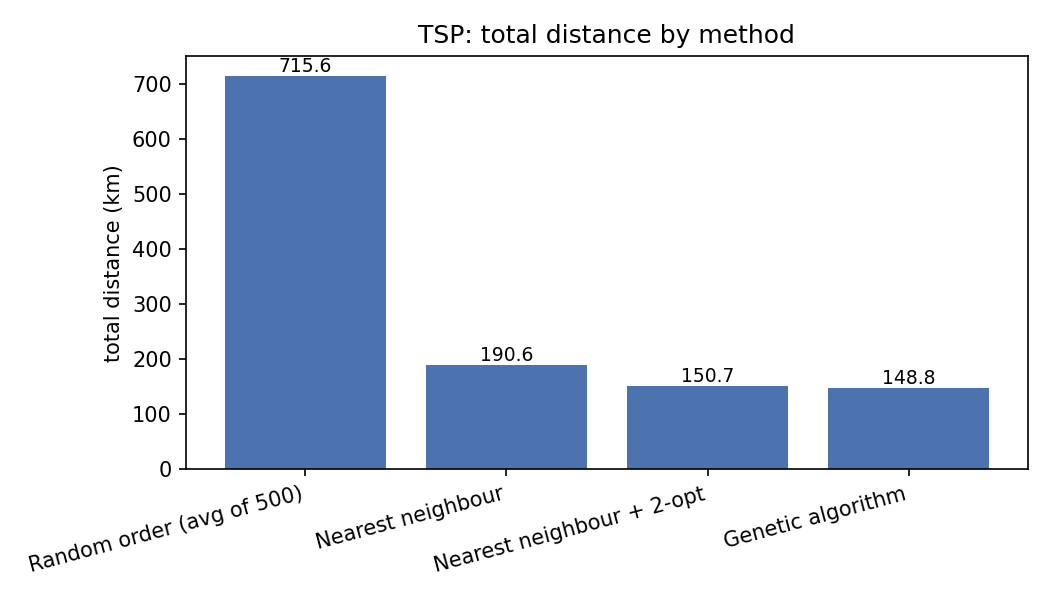
\includegraphics[width=0.85\linewidth]{tsp_comparison.png}
\caption{TSP tour length by method.}
\end{figure}

\subsection*{Observations}
\begin{itemize}
  \item \textbf{Any sensible method beats random order by a large margin.} Plain nearest neighbour already
        reduces the tour from 715.6~km to 190.6~km ($-73\%$).
  \item \textbf{2-opt is the best value.} It removes a further 20.9\% (190.55 to 150.74~km) in about 0.01~s.
  \item \textbf{The last few percent are expensive.} The genetic algorithm is only 1.3\% shorter than
        NN + 2-opt but takes roughly 1500 times longer. OR-Tools is 2.1\% shorter than NN + 2-opt and
        0.8\% shorter than the genetic algorithm, in about 10~s.
  \item \textbf{The genetic algorithm converges early.} In Figure~\ref{fig:ga} the best tour passes the
        NN + 2-opt level at around generation 100 and then flattens, with only two small improvements near
        generations 600 and 980. One thousand generations is more than this instance needs.
\end{itemize}

\begin{figure}[H]
\centering
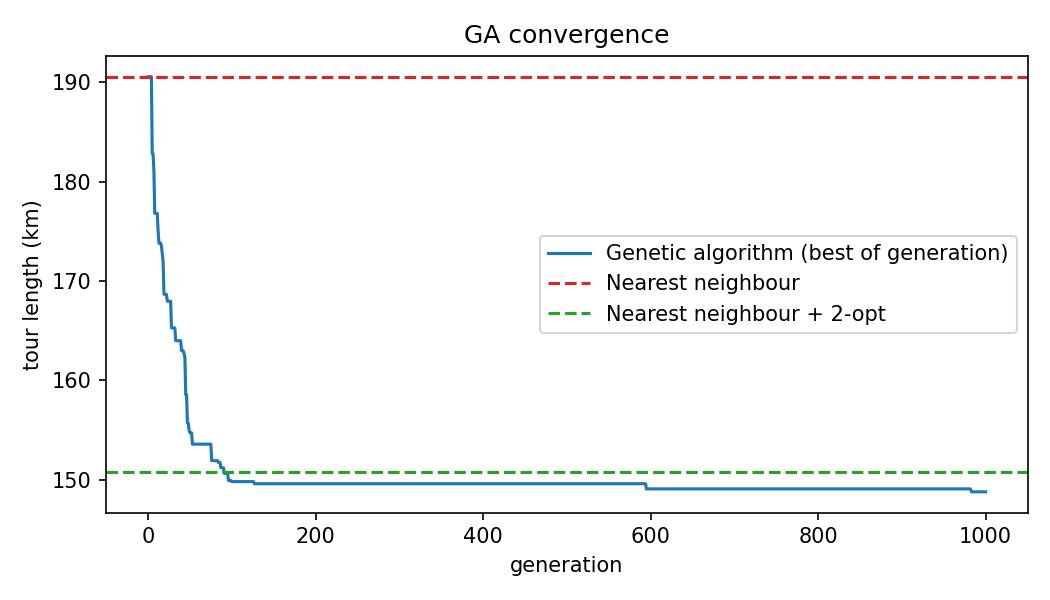
\includegraphics[width=0.8\linewidth]{ga_convergence.png}
\caption{Convergence of the genetic algorithm against the NN and NN + 2-opt tour lengths.}
\label{fig:ga}
\end{figure}

\paragraph{Conclusion.} OR-Tools gives the shortest tour (147.61~km), but NN + 2-opt is within 2.1\% of it
at almost no cost. The three best methods lie within about 2\% of each other, which suggests that the optimum
for this instance is close to 147~km (an observation, not a proof).

% ---------------- Part 2 ----------------
\section{Part 2: four vehicles, capacity 75 (CVRP)}

The fleet capacity is 300 parcels for a demand of 277, so the fleet is about 92\% full.

\begin{table}[H]
\centering
\begin{tabular}{lrrrr}
\toprule
Method & Distance (km) & Vehicles & Better than greedy & Runtime (s) \\
\midrule
Greedy capacity-aware NN  & 276.64 & 4 & --     & 0.00 \\
Greedy + 2-opt + relocate & 240.40 & 4 & 13.1\% & 0.00 \\
Sweep + 2-opt + relocate  & 210.33 & 4 & 24.0\% & 0.01 \\
Google OR-Tools           & \textbf{190.80} & 4 & 31.0\% & $\approx$10 \\
\bottomrule
\end{tabular}
\caption{CVRP results for 4 vehicles of capacity 75.}
\end{table}

\begin{figure}[H]
\centering
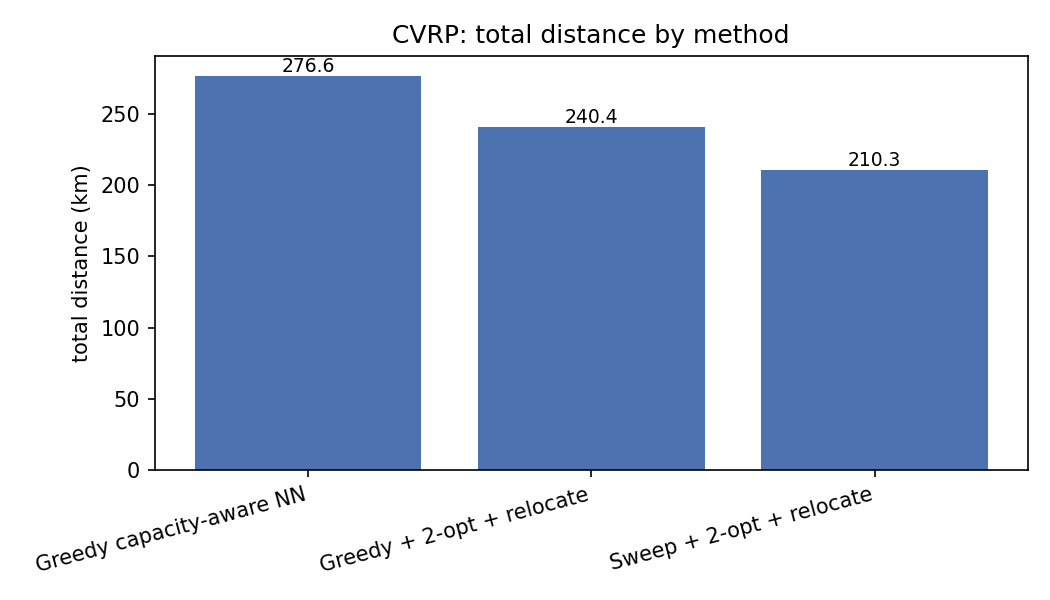
\includegraphics[width=0.85\linewidth]{vrp_comparison.png}
\caption{Total distance of the CVRP plans by method.}
\end{figure}

\subsection*{Observations}
\begin{itemize}
  \item \textbf{The starting solution matters a lot.} Local search improves both starting points, but the
        sweep start ends 12.5\% shorter than the greedy start (210.3 vs.\ 240.4~km). Sorting stops by
        angle around the depot gives compact, non-overlapping routes (Figure~\ref{fig:vrpbest}).
  \item \textbf{OR-Tools is 9.3\% shorter than the best heuristic} (190.8 vs.\ 210.3~km) and 31.0\% shorter
        than greedy. Sweep + local search closes most of the gap, but not all of it.
  \item \textbf{The OR-Tools routes are unbalanced in distance} (Table~\ref{tab:ortoolsroutes}). Vehicles~1
        and~2 drive about 55--58~km, vehicles~3 and~4 only about 38--40~km. The solver minimises total
        distance, not the longest route, so nothing pushes it to balance the vehicles. This matters in
        Part~3, because the day ends when the slowest vehicle returns.
  \item \textbf{Capacity is almost binding.} Vehicle~2 is exactly full and vehicle~3 is at 74/75.
\end{itemize}

\begin{table}[H]
\centering
\begin{tabular}{crrr}
\toprule
Vehicle & Stops & Load & Distance (km) \\
\midrule
1 & 11 & 70/75 & 57.7 \\
2 & 14 & 75/75 & 55.4 \\
3 & 12 & 74/75 & 37.6 \\
4 &  8 & 58/75 & 40.1 \\
\bottomrule
\end{tabular}
\caption{Best CVRP plan found by OR-Tools.}
\label{tab:ortoolsroutes}
\end{table}

\begin{figure}[H]
\centering
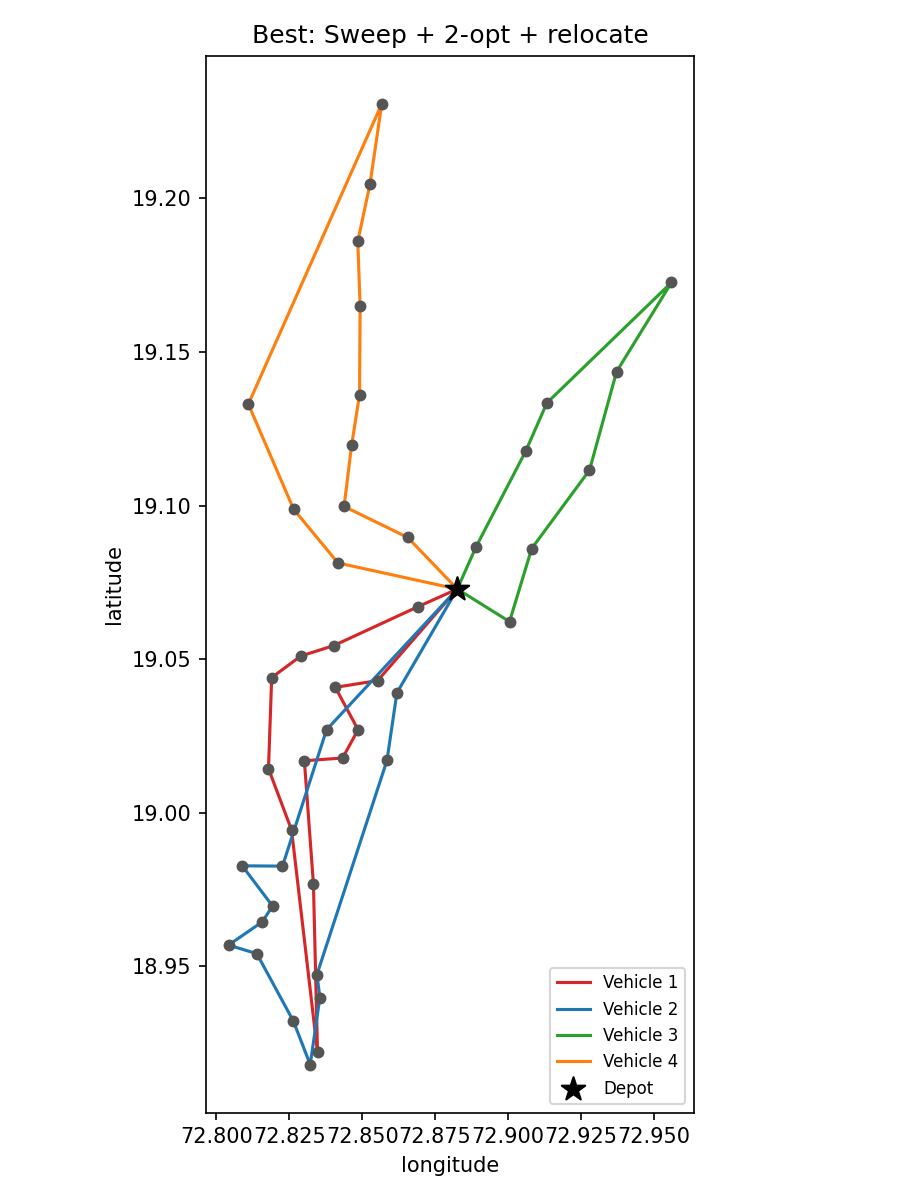
\includegraphics[height=9.5cm]{vrp_best.png}
\caption{Routes of the Sweep + 2-opt + relocate plan (4 vehicles, star = depot).}
\label{fig:vrpbest}
\end{figure}

\paragraph{Conclusion.} OR-Tools gives the lowest total distance (190.8~km). Where a simple method without
extra dependencies is preferred, sweep + 2-opt + relocate is a reasonable second choice at 10.2\% more distance than
OR-Tools.

% ---------------- Part 3 ----------------
\section{Part 3: Monte Carlo simulation}

Each plan was simulated for 2000 random days. The assumptions are 25~km/h base speed, rush-hour slowdowns,
rain on 15\% of days, random service times, 5\% failed deliveries and a 5.0~h shift. The ``finish'' time is
the time at which the last vehicle is back at the depot.

\begin{table}[H]
\centering
\footnotesize
\setlength{\tabcolsep}{3pt}
\begin{tabular}{lrrrrrrr}
\toprule
Method & Plan km & Route h & Finish h & P95 h & Overtime & OT h & Cost INR \\
\midrule
Greedy NN                 & 276.6 & 4.94 & 6.15 & 7.77 & 96.6\% & 1.91 & 9,797 \\
Greedy + 2-opt + relocate & 240.4 & 4.54 & 5.54 & 6.92 & 78.2\% & 0.84 & 9,095 \\
Sweep + 2-opt + relocate  & 210.3 & 4.16 & 4.65 & 5.76 & 21.1\% & 0.19 & 8,572 \\
Google OR-Tools           & 190.8 & 3.97 & 4.65 & 5.88 & 22.1\% & 0.19 & \textbf{8,336} \\
\bottomrule
\end{tabular}
\caption{Simulation results. Route h = mean route time, Finish h = mean finish time, P95 h = 95th percentile
of the finish time, Overtime = probability of exceeding the 5 h shift, OT h = mean overtime.}
\label{tab:sim}
\end{table}

\begin{figure}[H]
\centering
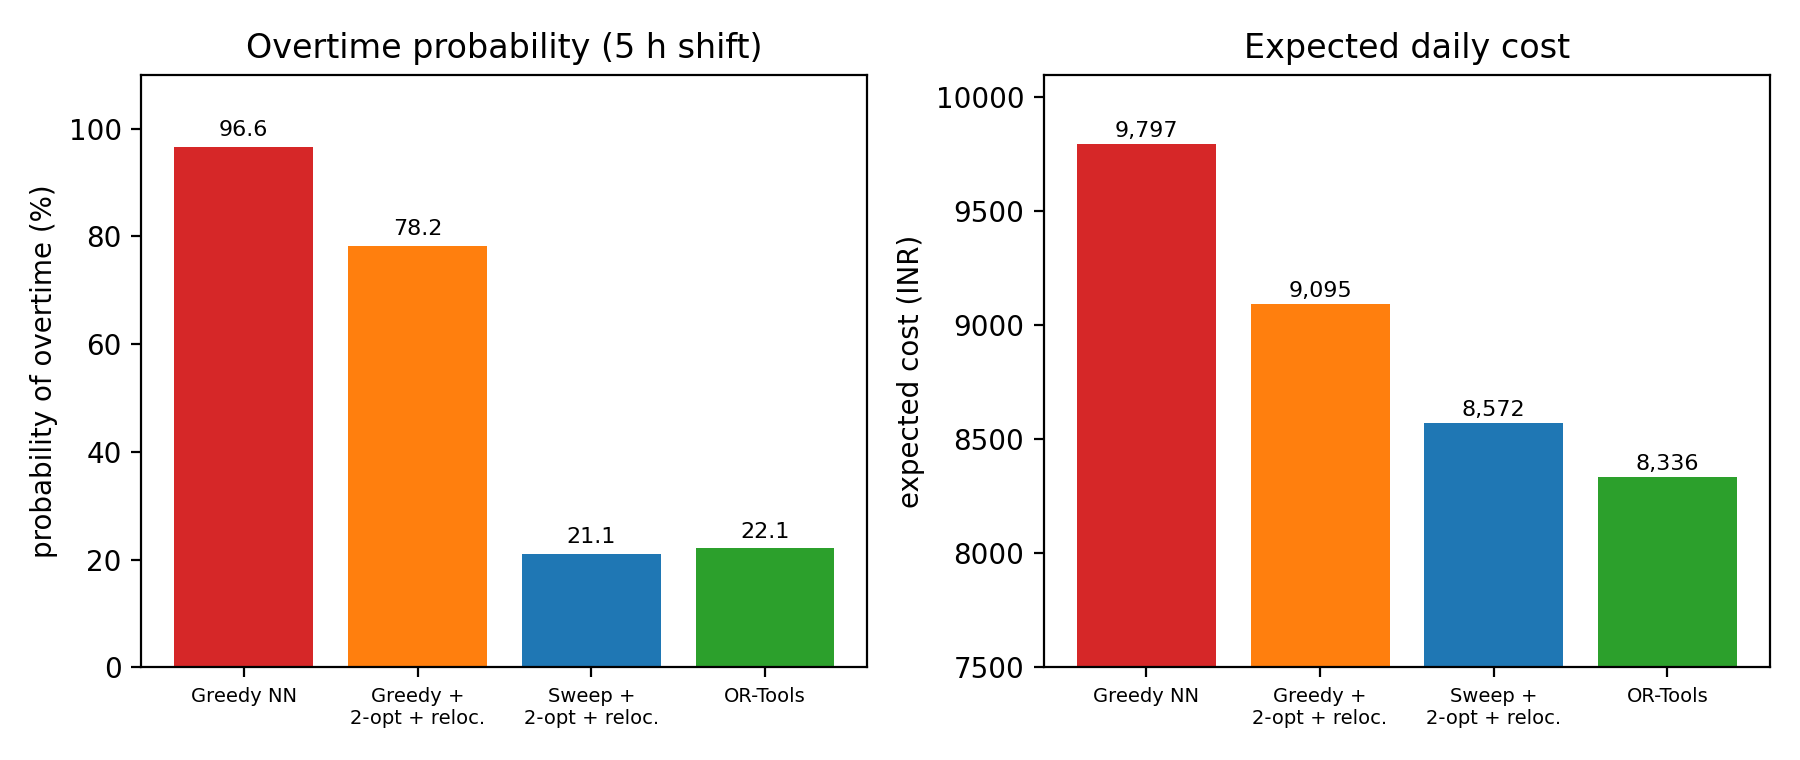
\includegraphics[width=\linewidth]{report_sim_methods.png}
\caption{Overtime probability and expected cost by method (drawn from the values in Table~\ref{tab:sim}).}
\end{figure}

\subsection*{Observations}
\begin{itemize}
  \item \textbf{Plan quality turns into operational risk.} A greedy plan ends after the 5~h shift on about
        97\% of simulated days (mean finish 6.15~h, P95 7.77~h). The sweep and OR-Tools plans reduce this to
        about 21--22\%.
  \item \textbf{A shorter plan helps less than the planned distance suggests.} OR-Tools plans 9.3\% fewer
        kilometres than Sweep, yet both have the same mean finish time (4.65~h) and almost the same overtime
        probability (22.1\% vs.\ 21.1\%). Sweep even has a slightly better P95 (5.76 vs.\ 5.88~h). The likely
        reason is the route imbalance seen in Part~2: the finish time is set by the longest route, and
        OR-Tools minimises total distance. This is an interpretation and was not tested directly.
  \item \textbf{OR-Tools still has the lowest expected cost} (8,336~INR), 14.9\% below greedy and 2.8\% below
        Sweep, so it remains the best choice on cost, although the margin over Sweep is small.
  \item \textbf{The ordering of the methods is stable.} Ranking by distance and by expected cost agree:
        greedy $<$ greedy + local search $<$ sweep $\approx$ OR-Tools.
\end{itemize}

% ---------------- Part 4 ----------------
\section{Fleet size what-if}

The sweep + 2-opt + relocate plan was re-run for 3 to 7 vehicles. The capacity per vehicle is scaled so that
the total fleet capacity is about 110\% of the demand (for example 3 $\times$ 102 or 7 $\times$ 44). The
4-vehicle row therefore uses capacity 77 instead of 75, but gives the same 210.3~km plan as Part~2.

\begin{table}[H]
\centering
\begin{tabular}{rrrrrr}
\toprule
Vehicles & Capacity & Plan km & P95 finish h & Overtime & Cost INR \\
\midrule
3 & 102 & 197.2 & 7.87 & 97.8\% &  7,224 \\
4 &  77 & 210.3 & 5.76 & 21.1\% &  8,572 \\
5 &  61 & 244.0 & 5.91 & 23.4\% & 10,473 \\
6 &  51 & 251.9 & 5.44 & 13.5\% & 12,038 \\
7 &  44 & 279.3 & 4.79 &  2.7\% & 13,855 \\
\bottomrule
\end{tabular}
\caption{Fleet size what-if for the sweep + 2-opt + relocate plan.}
\label{tab:fleet}
\end{table}

\begin{figure}[H]
\centering
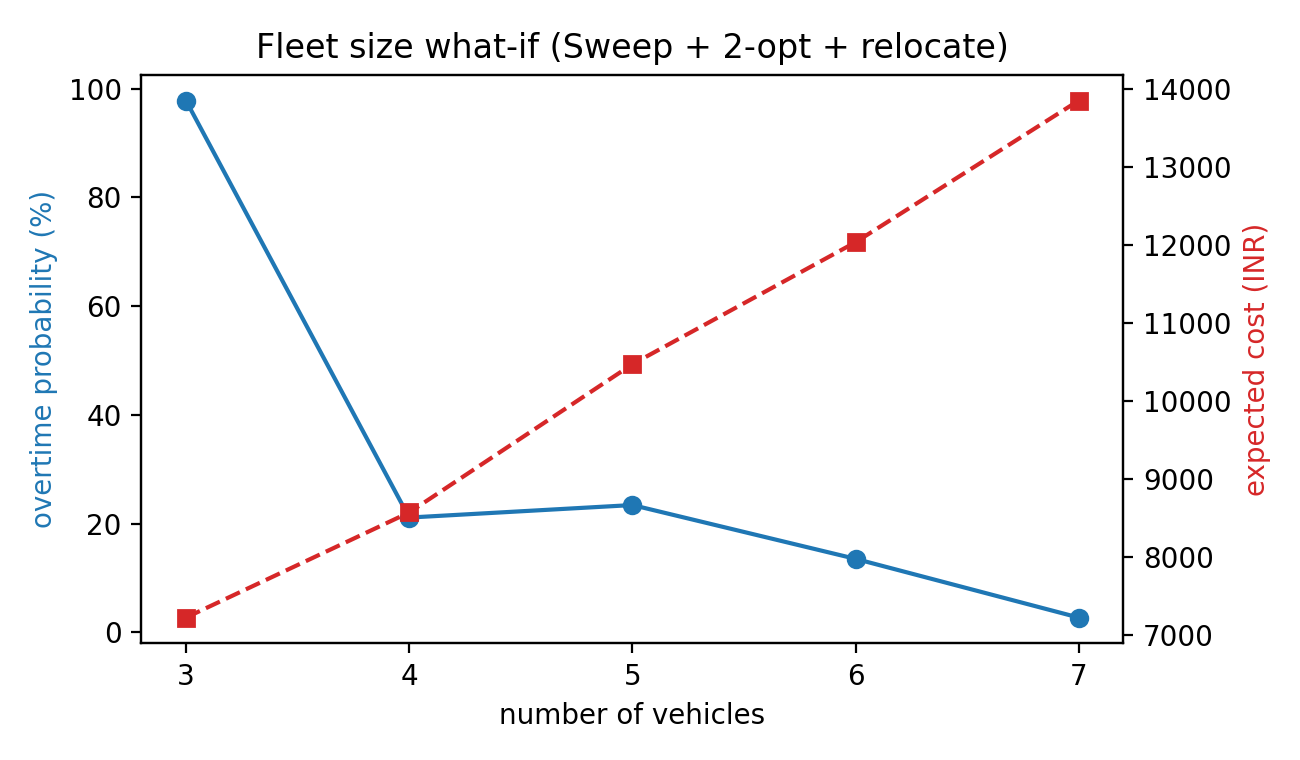
\includegraphics[width=0.75\linewidth]{report_fleet_whatif.png}
\caption{Overtime probability and expected cost against fleet size (drawn from Table~\ref{tab:fleet}).}
\end{figure}

\subsection*{Observations}
\begin{itemize}
  \item \textbf{Three vehicles are not feasible for a 5~h shift.} Overtime occurs on 97.8\% of days, even
        though it is the cheapest plan on paper.
  \item \textbf{Cost rises with every extra vehicle} (roughly 1,300 to 1,900~INR per vehicle). Planned
        kilometres also grow, because each vehicle makes its own trip out of and back to the Kurla depot.
  \item \textbf{Overtime falls with more vehicles, but not smoothly.} Six vehicles reduce it to 13.5\%
        and seven vehicles to 2.7\%. Reaching 2.7\% costs about 5,300~INR more per day than the 4-vehicle
        plan (13,855 vs.\ 8,572).
  \item \textbf{The 5-vehicle row is worse than the 4-vehicle row} (P95 5.91 vs.\ 5.76~h, overtime 23.4\% vs.\
        21.1\%), which should not happen with an extra vehicle. The most probable explanation is that the
        sweep heuristic produced an uneven split at that fleet size and left one long route. This is an
        artifact of the heuristic rather than a real effect, but it was not checked route by route.
\end{itemize}

\paragraph{Conclusion.} There is no free option. Four vehicles is the cheapest feasible plan but runs over
about one day in five. Seven vehicles nearly removes overtime but raises the cost by about 62\%. The right
choice depends on what an overtime day costs in practice.

% ---------------- Conclusions ----------------
\section{Overall conclusions}
\begin{enumerate}
  \item \textbf{Start with a good construction heuristic, then apply local search.} Sweep + 2-opt + relocate
        gets within about 10\% of OR-Tools on the CVRP, and NN + 2-opt within about 2\% on the TSP, in
        hundredths of a second.
  \item \textbf{OR-Tools gives the best plans in every comparison}, on distance and on expected cost, with a
        10~s time limit.
  \item \textbf{The genetic algorithm is not worth it here.} It is slower than OR-Tools and barely better than
        2-opt.
  \item \textbf{Minimum distance is not minimum risk.} Once randomness is added, the OR-Tools advantage
        shrinks. A formulation that balances route lengths, or minimises the longest route, is the obvious
        next experiment.
  \item \textbf{The 5~h shift is the binding constraint}, not vehicle capacity. Fleet size should be decided
        from the overtime and cost trade-off in the what-if table.
\end{enumerate}

\section{Suggested next steps}
\begin{itemize}
  \item Minimise the longest route, or add a balance penalty, in OR-Tools and re-run the simulation.
  \item Inspect the 5-vehicle sweep solution to confirm the uneven-split explanation.
  \item Repeat the study with real OSRM road distances and with several seeds to obtain confidence intervals.
  \item Test larger instances (100+ stops), where OR-Tools and the simple heuristics are likely to diverge more.
\end{itemize}

\end{document}
